\section{Azure Backup performance tests}
\label{app:chab-perf}
Four attempts were made at recovering the VM with Azure Backup.
The first two failed, presumably because something was wrong with the restore point used.

The two last attempts used a different restore point.
The time spent was measured using a stopwatch.
Measurements were started the moment the restore job was started
and stopped when it was possible to SSH to the VM and query the database.

Azure measures the time taken by the restore job itself.
This is noted separately.
The total time is influenced by how fast we were able to paste commands into the CLI.
The restore job time is probably the most interesting time.

Recovery using Azure Portal:
\begin{center}
\begin{tabular}{lr}
\hline
 & Time (hours:minutes:seconds)\\
\hline
Restore job: & 00:02:10\\
Total: & 00:03:30\\
\hline
\end{tabular}
\end{center}

Recovery using Azure CLI:
\begin{center}
\begin{tabular}{lr}
\hline
 & Time (hours:minutes:seconds)\\
\hline
Restore job: & 00:01:06\\
Total: & 00:06:33\\
\hline
\end{tabular}
\end{center}


\subsection{Recovery with Azure Backup via CLI (failed first attempt)}
\label{sec:orgb039355}
\subsubsection{Delete VM}
\label{sec:org5859260}
There are not enough vCPUs available in the quota,
which means the VM has to be deleted before recovery can happen.

\begin{minted}[breaklines=true,breakanywhere=true]{powershell}
az vm delete --name $CHName --resource-group $RGName --yes
\end{minted}

\subsubsection{Preparation}
\label{sec:orgd393ff5}
Prepare environment and retrieve restore points
\begin{minted}[breaklines=true,breakanywhere=true]{powershell}
# Get RSV and set context
$RSV = Get-AzRecoveryServicesVault -Name $RSVName -ResourceGroupName $RGName
Set-AzRecoveryServicesVaultContext -Vault $RSV

# Select VM
$namedContainer = Get-AzRecoveryServicesBackupContainer  -ContainerType "AzureVM" -Status "Registered" -FriendlyName $CHName -VaultId $RSV.ID
$backupitem = Get-AzRecoveryServicesBackupItem -Container $namedContainer  -WorkloadType "AzureVM" -VaultId $RSV.ID

# Get start and end date
$startDate = (Get-Date).AddDays(-7)
$endDate = Get-Date

# Store recovery points in variable
$rp = Get-AzRecoveryServicesBackupRecoveryPoint -Item $backupitem -StartDate $startdate.ToUniversalTime() -EndDate $enddate.ToUniversalTime() -VaultId $RSV.ID
\end{minted}

List contents of \texttt{\$rp}:
\begin{minted}[breaklines=true,breakanywhere=true]{powershell}
$rp
# RecoveryPointId    RecoveryPointType  RecoveryPointTime      ContainerName                        ContainerType
# ---------------    -----------------  -----------------      -------------                        -------------
# 15649757922643     FileSystemConsist… 5/11/2022 7:44:53 PM   iaasvmcontainerv2;perfrg;perfclickh… AzureVM
# 12290901249728     FileSystemConsist… 5/11/2022 11:09:00 AM  iaasvmcontainerv2;perfrg;perfclickh… AzureVM
\end{minted}

12290901249728 is the point that was triggered manually when Azure Backup was set up (see \ref{app:ch-perf}).
The point is stored in \texttt{\$rp[1]}.

\subsubsection{Create restore job}
\label{sec:orgd99419b}
Start restore job:
\begin{minted}[breaklines=true,breakanywhere=true]{powershell}
# Select recovery point
$RecPoint = $rp[1]

# Create a restore job for the backup item
$restorejob = Restore-AzRecoveryServicesBackupItem -RecoveryPoint $RecPoint -StorageAccountName $StagingSAName -StorageAccountResourceGroupName $RGName -TargetResourceGroupName $RGName -VaultId $RSV.ID

# Wait for the restore job to complete
Wait-AzRecoveryServicesBackupJob -Job $restorejob -Timeout 43200
# WorkloadName     Operation            Status               StartTime                 EndTime                   JobID
# ------------     ---------            ------               ---------                 -------                   -----
# perfclickhousevm Restore              Completed            5/12/2022 7:13:45 AM      5/12/2022 7:14:51 AM      30d32412-e718-4dde-a52e-c48444364cf3

# Get details of the restore job
$restorejob = Get-AzRecoveryServicesBackupJob -Job $restorejob -VaultId $RSV.ID
$details = Get-AzRecoveryServicesBackupJobDetail -Job $restorejob -VaultId $RSV.ID
\end{minted}

Contents of \texttt{\$details.Properties}:
\begin{minted}[breaklines=true,breakanywhere=true]{powershell}
$details.Properties

# Key                         Value
# ---                         -----
# Job Type                    Recover disks
# Target VM Name              vmName
# Target Storage Account Name perfstagingchsa
# Recovery point time         5/11/2022 11:09:00 AM
# Config Blob Name            config-perfclickhousevm-30d32412-e718-4dde-a52e-c48444364cf3.json
# Config Blob Container Name  perfclickhousevm-8726c9fbe67e4ca4a5ff7e06238eac29
# Config Blob Uri             https://perfstagingchsa.blob.core.windows.net/perfclickhousevm-8726c9fbe67e4ca4a5ff7e06238eac29/config-perfclickhousevm-30d32412-e718-4dde-a52e-c48444364cf3.json
# Target resource group       perfRG
# Template Blob Uri           https://perfstagingchsa.blob.core.windows.net/perfclickhousevm-8726c9fbe67e4ca4a5ff7e06238eac29/azuredeploy30d32412-e718-4dde-a52e-c48444364cf3.json
\end{minted}

Save details:
\begin{minted}[breaklines=true,breakanywhere=true]{powershell}
$properties = $details.properties
$storageAccountName = $properties["Target Storage Account Name"]
$containerName = $properties["Config Blob Container Name"]
$templateBlobURI = $properties["Template Blob Uri"]
\end{minted}

\subsubsection{Deploy VM}
\label{sec:orgd09ce0a}
Deploy VM:
\begin{minted}[breaklines=true,breakanywhere=true]{powershell}
# Template name was copied from the last part of "Template Blob Uri"
$templateName = "azuredeploy30d32412-e718-4dde-a52e-c48444364cf3.json"

# Set the storage account
Set-AzCurrentStorageAccount -Name $storageAccountName -ResourceGroupName $RGName

# Generate SAS token
$templateBlobFullURI = New-AzStorageBlobSASToken -Container $containerName -Blob $templateName -Permission r -FullUri

# Deploy VM (VirtualMachineName had to be specified interactively)
New-AzResourceGroupDeployment -Name $CHName -ResourceGroupName $RGName -TemplateUri $templateBlobFullURI
#DeploymentName          : perfClickhouseVM
#ResourceGroupName       : perfRG
#ProvisioningState       : Succeeded
#Timestamp               : 5/12/2022 7:20:25 AM
#Mode                    : Incremental
#TemplateLink            :
#         Uri            : https://perfstagingchsa.blob.core.windows.net/perfclickhousevm-8726c9fbe67e4ca4a5ff7e06238eac29/azuredeploy30d32412-e718-4dde-a52e-c48444364cf3.json?sv=2021-04-10&se=2022-05-12T08%3A19%3A11Z&sr=b&sp=r
#         &sig=5Uzo66b%2B1I9IvrpVokKaqHtJiBCx0ZEl6r8SIyM0XGc%3D
#         ContentVersion : 1.0.0.0
#
#Parameters              :
# Name                           Type                       Value
# =============================  =========================  ==========
# virtualMachineName             String                     "perfClickhouseVM"
# virtualNetwork                 String                     "perfClickhouseVMVNET"
# virtualNetworkResourceGroup    String                     "perfRG"
# subnet                         String                     "perfClickhouseVMSubnet"
# osDiskName                     String                     "perfClickhouseVMOSDisk"
# networkInterfacePrefixName     String                     "perfClickhouseVMRestoredNIC"
# publicIpAddressName            String                     "perfClickhouseVMRestoredip"
#
#Outputs                 :
#DeploymentDebugLogLevel :
\end{minted}

\subsubsection{Trouble connecting to the VM}
\label{sec:org3c86200}
\texttt{clickhouse-client} would not start at first.
The VM was therefore restarted.
After this, SSH would time out repeatedly.
The VM was restarted again, but SSH still did not work.
Azure's SSH ``Connection troubleshoot'' in the Azure Portal was attempted,
but it would also hang for a long time.

Another attempt at recovering the data was attempted with the Azure Portal.
The recovery appears to have succeeded.
The same problems with \texttt{clickhouse-client} not starting,
and SSH timing out still appeared, though.
Maybe the restore point was broken in some way.

We decided to abort the attempt at recovering with Azure Backup for now.
Instead, we decided to try to recover with \texttt{clickhouse-backup} instead,
and then make a new restore point in Azure Backup to recover from.

\subsection{Recovery with Azure Backup (failed second attempt)}
\label{sec:org2c0f303}
We tried to recover from Azure Backup once again.
Output was omitted for brevity, except for when waiting for the restore job,
as that output contains information about the time the restore job took.

\subsubsection{Delete VM}
\label{sec:org0fbc45f}
\begin{minted}[breaklines=true,breakanywhere=true]{powershell}
az vm delete --name $CHName --resource-group $RGName --yes
\end{minted}

\subsubsection{Get restore point}
\label{sec:orgd8ba7ae}
\begin{minted}[breaklines=true,breakanywhere=true]{powershell}
# Get RSV and set context
$RSV = Get-AzRecoveryServicesVault -Name $RSVName -ResourceGroupName $RGName
Set-AzRecoveryServicesVaultContext -Vault $RSV

# Select VM
$namedContainer = Get-AzRecoveryServicesBackupContainer  -ContainerType "AzureVM" -Status "Registered" -FriendlyName $CHName -VaultId $RSV.ID
$backupitem = Get-AzRecoveryServicesBackupItem -Container $namedContainer  -WorkloadType "AzureVM" -VaultId $RSV.ID

# Get start and end date
$startDate = (Get-Date).AddDays(-7)
$endDate = Get-Date

# Store recovery points in variable
$rp = Get-AzRecoveryServicesBackupRecoveryPoint -Item $backupitem -StartDate $startdate.ToUniversalTime() -EndDate $enddate.ToUniversalTime() -VaultId $RSV.ID
\end{minted}

\subsubsection{Restore}
\label{sec:org22dad73}
Start restore job:
\begin{minted}[breaklines=true,breakanywhere=true]{powershell}
# Select recovery point
$RecPoint = $rp[1]

# Create a restore job for the backup item
$restorejob = Restore-AzRecoveryServicesBackupItem -RecoveryPoint $RecPoint -StorageAccountName $StagingSAName -StorageAccountResourceGroupName $RGName -TargetResourceGroupName $RGName -VaultId $RSV.ID

# Wait for the restore job to complete
Wait-AzRecoveryServicesBackupJob -Job $restorejob -Timeout 43200
# WorkloadName     Operation            Status               StartTime                 EndTime                   JobID
# ------------     ---------            ------               ---------                 -------                   -----
# perfclickhousevm Restore              Completed            5/12/2022 11:30:24 AM     5/12/2022 11:31:34 AM     2940f1d3-b57f-4428-9b1b-066e116a1389

# Get details of the restore job
$restorejob = Get-AzRecoveryServicesBackupJob -Job $restorejob -VaultId $RSV.ID
$details = Get-AzRecoveryServicesBackupJobDetail -Job $restorejob -VaultId $RSV.ID
\end{minted}

Save details:
\begin{minted}[breaklines=true,breakanywhere=true]{powershell}
$properties = $details.properties
$storageAccountName = $properties["Target Storage Account Name"]
$containerName = $properties["Config Blob Container Name"]
$templateBlobURI = $properties["Template Blob Uri"]
\end{minted}

\subsubsection{Deploy VM (failed)}
\label{sec:org9eacaf3}
Deploy VM:
\begin{minted}[breaklines=true,breakanywhere=true]{powershell}
# Template name was copied from the last part of "Template Blob Uri"
$templateName = "azuredeploy2940f1d3-b57f-4428-9b1b-066e116a1389.json"

# Set the storage account
Set-AzCurrentStorageAccount -Name $storageAccountName -ResourceGroupName $RGName

# Generate SAS token
$templateBlobFullURI = New-AzStorageBlobSASToken -Container $containerName -Blob $templateName -Permission r -FullUri

# Deploy VM (VirtualMachineName had to be specified interactively)
New-AzResourceGroupDeployment -Name $CHName -ResourceGroupName $RGName -TemplateUri $templateBlobFullURI
# New-AzResourceGroupDeployment: 11:34:35 AM - The deployment 'perfClickhouseVM' failed with error(s). Showing 1 out of 1 error(s).
# Status Message: Resource /subscriptions/4b48eb85-91f3-4902-b74b-e84641fb6785/resourceGroups/perfRG/providers/Microsoft.Network/networkInterfaces/perfClickhouseVMRestoredNIC5324890b7fe44a77ae9def7a461b6e81/ipConfigurations/c0dbf1d5514749ec849957897d9405d1 is referencing public IP address /subscriptions/4b48eb85-91f3-4902-b74b-e84641fb6785/resourceGroups/perfRG/providers/Microsoft.Network/publicIPAddresses/perfClickhouseVMRestoredip that is already allocated to resource /subscriptions/4b48eb85-91f3-4902-b74b-e84641fb6785/resourceGroups/perfRG/providers/Microsoft.Network/networkInterfaces/perfClickhouseVMRestoredNICb9bd95260138425bab106f324a42acbc/ipConfigurations/7ba12bb4efcf444d9f08dd1aff9a1cc6. (Code: PublicIPAddressInUse)
# CorrelationId: 2677f822-ff57-4405-8600-c96b2eb802b4
#
# DeploymentName          : perfClickhouseVM
# ResourceGroupName       : perfRG
# ProvisioningState       : Failed
# Timestamp               : 5/12/2022 11:34:30 AM
# Mode                    : Incremental
# TemplateLink            :
#                           Uri            : https://perfstagingchsa.blob.core.windows.net/perfclickhousevm-b52ea1d968e04fc68ea92dea4d441451/azuredeploy2940f1d3-b57f-4428-9b1b-066e116a1389.json?sv=2
#                           021-04-10&se=2022-05-12T12%3A33%3A08Z&sr=b&sp=r&sig=ELTwTiFCjOc3kLiTipWd0cElPgJcGFidk8EXxJxaYfU%3D
#                           ContentVersion : 1.0.0.0
#
# Parameters              :
#                           Name                           Type                       Value
#                           =============================  =========================  ==========
#                           virtualMachineName             String                     "perfClickhouseVM"
#                           virtualNetwork                 String                     "perfClickhouseVMVNET"
#                           virtualNetworkResourceGroup    String                     "perfRG"
#                           subnet                         String                     "perfClickhouseVMSubnet"
#                           osDiskName                     String                     "perfClickhouseVMOSDisk"
#                           networkInterfacePrefixName     String                     "perfClickhouseVMRestoredNIC"
#                           publicIpAddressName            String                     "perfClickhouseVMRestoredip"
#
# Outputs                 :
\end{minted}

The deployment failed because the IP address was consider to already be in use.
The Azure Portal seems to be able to deal with these kinds of conflicts better,
so we tried to deploy using the Portal.

\subsubsection{Deploy VM using the Azure Portal}
\label{sec:org9b58952}
We decided to try to restore the VM using the Azure Portal,
instead of the CLI.

Restoring the VM using the Azure Portal:
\begin{center}
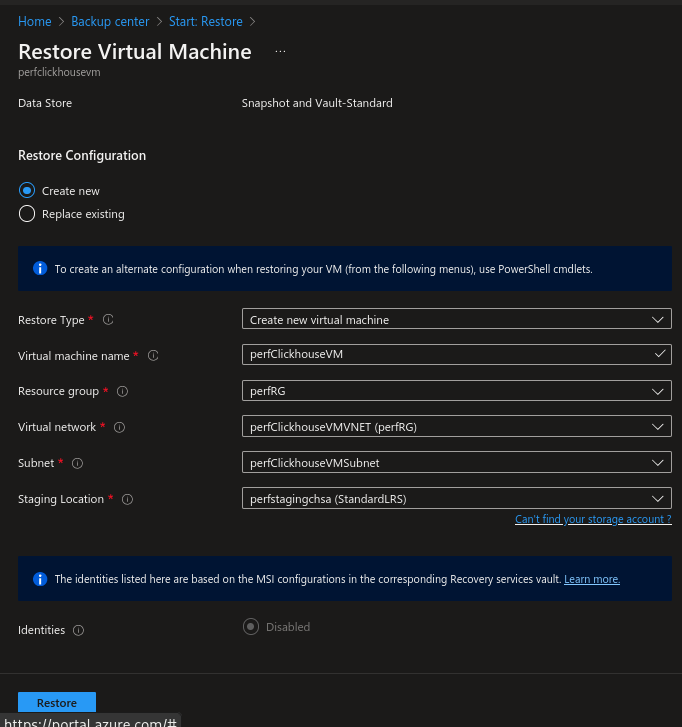
\includegraphics[width=.9\linewidth]{figures/clickhouse/azure_restore_portal.png}
\end{center}

According to the Azure Portal, the duration of the restore
was 2 minutes and 15 seconds.

Details for the restore job:
\begin{center}
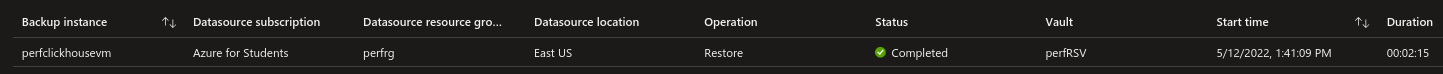
\includegraphics[width=.9\linewidth]{figures/clickhouse/ab_restore_duration.png}
\end{center}

\subsubsection{Connect to VM and verify recovery}
\label{sec:org7097732}
At first \texttt{clickhouse-client} would not start.
Several attempt were made at starting or restarting the ClickHouse server with
\texttt{sudo systemctl [start/restart] clickhouse-server.service}.

We attempted to reboot the VM.
After that, we experienced the same problem as earlier, where SSH would not connect.

After a lot of troubleshooting, we gave up.

\subsection{Recovery with Azure Backup via Portal (successful third attempt)}
\label{sec:org1aa719c}
The VM was first deleted using the Azure Portal.

The VM was then restored from a different restore point
(one that was automatically created on the same day, but later).

Restoring the VM:
\begin{center}
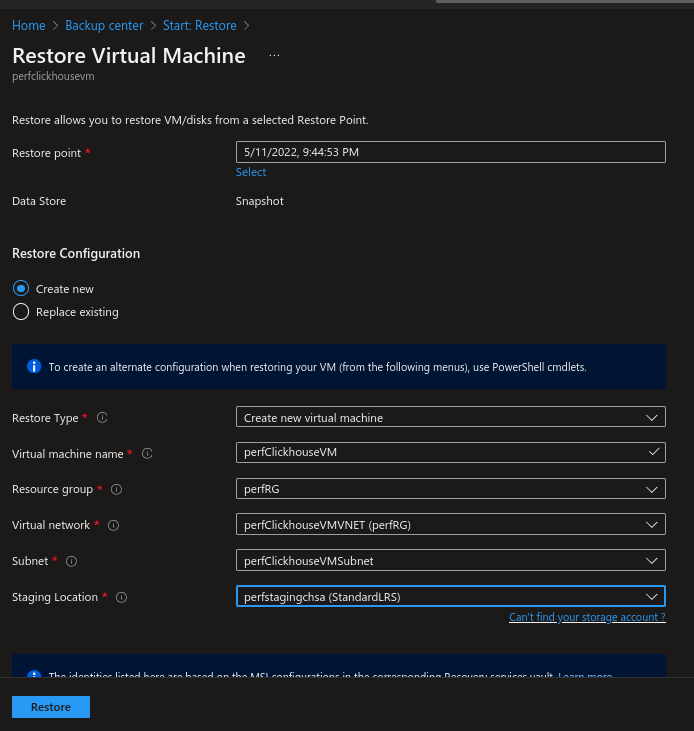
\includegraphics[width=.9\linewidth]{figures/clickhouse/ab_restore_2.png}
\end{center}

The duration was 2 minutes, 10 seconds:
\begin{center}
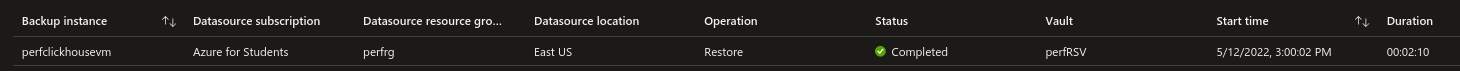
\includegraphics[width=.9\linewidth]{figures/clickhouse/ab_restore2_duration.png}
\end{center}

We were able to connect to the VM immediately.
\texttt{clickhouse-client} would not start on the first boot.
The server was rebooted.
After this, \texttt{clickhouse-client} started like normal.
It took 1 minutes and 20 seconds to get \texttt{clickhouse-client} up and running after the restore job.
The total time for the entire restoration was 3 minutes and 30 seconds.

Listing the table sizes:
\begin{minted}[breaklines=true,breakanywhere=true]{sql}
SELECT
    database,
    table,
    formatReadableSize(sum(data_compressed_bytes) AS size) AS compressed,
    formatReadableSize(sum(data_uncompressed_bytes) AS usize) AS uncompressed,
    round(usize / size, 2) AS compr_rate,
    sum(rows) AS rows,
    count() AS part_count
FROM system.parts
WHERE (active = 1) AND (database LIKE '%') AND (table LIKE '%')
GROUP BY
    database,
    table
ORDER BY size DESC
\end{minted}

Result:
\begin{center}
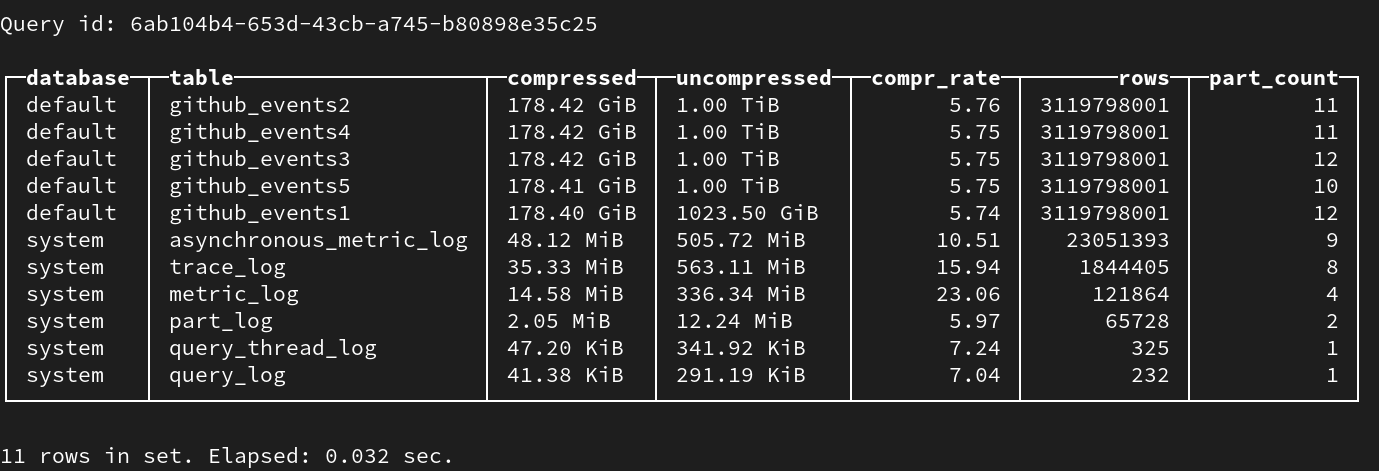
\includegraphics[width=.9\linewidth]{figures/clickhouse/ab_restore2_tables.png}
\end{center}

Everything appears to be in order.

\subsection{Recovery with Azure Backup via CLI (successful fourth attempt)}
\label{sec:orgcd90f70}
We decided to try to recover the VM via the CLI one last time,
this time using the same restore point as we did in the successful
attempt where we used the Azure Portal.

The restore job itself took 1 minute and 6 seconds.
The total time was 6 minutes and 33 seconds.

\subsubsection{Preparation}
\label{sec:org012927e}
Delete VM:
\begin{minted}[breaklines=true,breakanywhere=true]{powershell}
az vm delete --name $CHName --resource-group $RGName --yes
\end{minted}

Prepare environment and retrieve restore points
\begin{minted}[breaklines=true,breakanywhere=true]{powershell}
# Get RSV and set context
$RSV = Get-AzRecoveryServicesVault -Name $RSVName -ResourceGroupName $RGName
Set-AzRecoveryServicesVaultContext -Vault $RSV

# Select VM
$namedContainer = Get-AzRecoveryServicesBackupContainer  -ContainerType "AzureVM" -Status "Registered" -FriendlyName $CHName -VaultId $RSV.ID
$backupitem = Get-AzRecoveryServicesBackupItem -Container $namedContainer  -WorkloadType "AzureVM" -VaultId $RSV.ID

# Get start and end date
$startDate = (Get-Date).AddDays(-7)
$endDate = Get-Date

# Store recovery points in variable
$rp = Get-AzRecoveryServicesBackupRecoveryPoint -Item $backupitem -StartDate $startdate.ToUniversalTime() -EndDate $enddate.ToUniversalTime() -VaultId $RSV.ID
\end{minted}

List contents of \texttt{\$rp}:
\begin{minted}[breaklines=true,breakanywhere=true]{powershell}
$rp
# RecoveryPointId    RecoveryPointType  RecoveryPointTime      ContainerName                        ContainerType
# ---------------    -----------------  -----------------      -------------                        -------------
# 15649757922643     FileSystemConsist… 5/11/2022 7:44:53 PM   iaasvmcontainerv2;perfrg;perfclickh… AzureVM
# 12290901249728     FileSystemConsist… 5/11/2022 11:09:00 AM  iaasvmcontainerv2;perfrg;perfclickh… AzureVM
\end{minted}

Since we were able to restore the VM using \texttt{\$rp[0]} (15649757922643),
when using the Azure Portal, we decided to try using it with the CLI as well.

\subsubsection{Create restore job}
\label{sec:org58fc843}
A stopwatch was started the moment the restore job was initiated.

\begin{minted}[breaklines=true,breakanywhere=true]{powershell}
# Select recovery point
$RecPoint = $rp[0]

# Create a restore job for the backup item
$restorejob = Restore-AzRecoveryServicesBackupItem -RecoveryPoint $RecPoint -StorageAccountName $StagingSAName -StorageAccountResourceGroupName $RGName -TargetResourceGroupName $RGName -VaultId $RSV.ID

# Wait for the restore job to complete
Wait-AzRecoveryServicesBackupJob -Job $restorejob -Timeout 43200
# WorkloadName     Operation            Status               StartTime                 EndTime                   JobID
# ------------     ---------            ------               ---------                 -------                   -----
# perfclickhousevm Restore              Completed            5/12/2022 1:29:59 PM      5/12/2022 1:31:05 PM      17882329-4b0f-416f-8080-bbfd7a32f81b

# Get details of the restore job
$restorejob = Get-AzRecoveryServicesBackupJob -Job $restorejob -VaultId $RSV.ID
$details = Get-AzRecoveryServicesBackupJobDetail -Job $restorejob -VaultId $RSV.ID
\end{minted}

The restore job lasted from 1:29:59 PM to 1:31:05 PM,
which means the duration was 1 minute and 6 seconds.

Save details:
\begin{minted}[breaklines=true,breakanywhere=true]{powershell}
$properties = $details.properties
$storageAccountName = $properties["Target Storage Account Name"]
$containerName = $properties["Config Blob Container Name"]
$templateBlobURI = $properties["Template Blob Uri"]
\end{minted}

\subsubsection{Deploy VM}
\label{sec:orgf121154}
Generate SAS:
\begin{minted}[breaklines=true,breakanywhere=true]{powershell}
# Template name was copied from the last part of "Template Blob Uri"
$templateName = "azuredeploy17882329-4b0f-416f-8080-bbfd7a32f81b.json"

# Set the storage account
Set-AzCurrentStorageAccount -Name $storageAccountName -ResourceGroupName $RGName

# Generate SAS token
$templateBlobFullURI = New-AzStorageBlobSASToken -Container $containerName -Blob $templateName -Permission r -FullUri
\end{minted}

Deploy VM:
\begin{minted}[breaklines=true,breakanywhere=true]{powershell}
# Deploy VM (VirtualMachineName had to be specified interactively)
New-AzResourceGroupDeployment -Name $CHName -ResourceGroupName $RGName -TemplateUri $templateBlobFullURI
#DeploymentName          : perfClickhouseVM
#ResourceGroupName       : perfRG
#ProvisioningState       : Succeeded
#Timestamp               : 5/12/2022 1:38:51 PM
#Mode                    : Incremental
#TemplateLink            :
#                          Uri            : https://perfstagingchsa.blob.core.windows.net/perfclickhousevm-0411d36fae58488d809caa803c51a60a/azuredeploy17882329-4b0f-416f-8080-bbfd7a32f81b.json?sv=2
#                          021-04-10&se=2022-05-12T14%3A36%3A06Z&sr=b&sp=r&sig=xIXTM%2FIAZW40zO5nv%2BRFcB4MJrNeAhaLbYWo4oMHKz0%3D
#                          ContentVersion : 1.0.0.0
#
#Parameters              :
#                          Name                           Type                       Value
#                          =============================  =========================  ==========
#                          virtualMachineName             String                     "perfClickhouseVM"
#                          virtualNetwork                 String                     "perfClickhouseVMVNET"
#                          virtualNetworkResourceGroup    String                     "perfRG"
#                          subnet                         String                     "perfClickhouseVMSubnet"
#                          osDiskName                     String                     "perfClickhouseVMOSDisk"
#                          networkInterfacePrefixName     String                     "perfClickhouseVMRestoredNIC"
#                          publicIpAddressName            String                     "perfClickhouseVMRestoredip"
#
#Outputs                 :
#DeploymentDebugLogLevel :
\end{minted}

\subsubsection{Verify that the recovery was successful}
\label{sec:org7d71d01}
We were able to connect to the VM with SSH after 4 minutes and 49 seconds.
\texttt{clickhouse-client} would not start on the first boot.
The VM was restarted.
After this, \texttt{clickhouse-client} started properly and we were able to query the database.
The total time was 6 minutes and 33 seconds.

Listing the table sizes:
\begin{minted}[breaklines=true,breakanywhere=true]{sql}
SELECT
    database,
    table,
    formatReadableSize(sum(data_compressed_bytes) AS size) AS compressed,
    formatReadableSize(sum(data_uncompressed_bytes) AS usize) AS uncompressed,
    round(usize / size, 2) AS compr_rate,
    sum(rows) AS rows,
    count() AS part_count
FROM system.parts
WHERE (active = 1) AND (database LIKE '%') AND (table LIKE '%')
GROUP BY
    database,
    table
ORDER BY size DESC
\end{minted}

Result:
\begin{center}
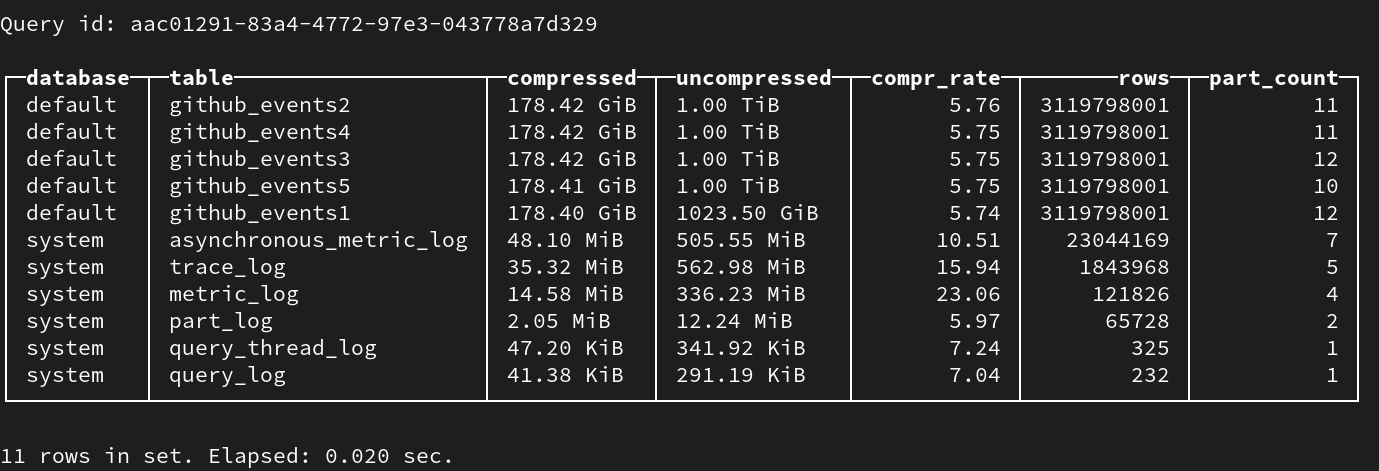
\includegraphics[width=.9\linewidth]{figures/clickhouse/restore3_tables.png}
\end{center}

It appears that the recovery was successful!
